\scanpage{78}
% archive foliation: 77
% top, unfinished formula
\[\rho_0=\]
% upper-left incidence diagram
\diagram{\begin{tikzcd}[ampersand replacement=\&,column sep=small,row sep=small]
\&\&E^+\arrow[dddll]\arrow[dddrr]\arrow[d]\arrow[ddl,"\pi_2^+"']\arrow[ddr,"\pi_1^+"]\arrow[ddd,dash,bend right=4,"\pi_0^+"]\&\&\\
\&\&\deleted{D_{12}}D_{12}\arrow[ddrr,dash]\&\&\\
\&S_2\&\&S_1\&\\
D_{20}\arrow[uurr,dash]\arrow[rrrr,dash]\&\&S_0\&\&D_{01}\\
\&\&E^-\arrow[ull,dash]\arrow[urr,dash]\arrow[uuu,bend left=5]\arrow[uul,"\pi_2^-"']\arrow[uur,"\pi_1^-"]\arrow[u,"\pi_0^-"']\&\&
\end{tikzcd}}
% middle-right polygon drawing
\figure{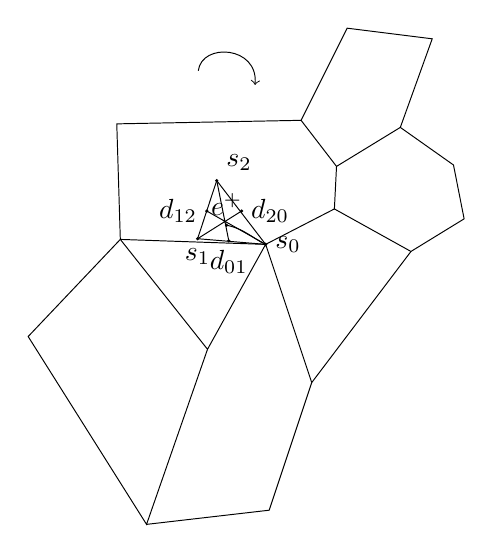
\begin{tikzpicture}[x=.009cm,y=-.009cm,line width=.35pt]
\draw (920,815)--(1180,810)--(1230,875)--(1227,935)--(1130,985)--(925,978)--cycle;
\draw (1180,810)--(1245,680)--(1365,695)--(1320,820)--(1230,875);
\draw (1320,820)--(1395,873)--(1410,949)--(1335,995)--(1227,935);
\draw (925,978)--(1048,1133)--(1130,985)--(1195,1180)--(1335,995);
\draw (925,978)--(795,1115)--(962,1380)--(1048,1133);
\draw (962,1380)--(1135,1360)--(1195,1180);
\draw[->] (1035,740) .. controls (1040,700) and (1120,705) .. (1115,760);
\coordinate (a) at (1034,977);\coordinate (b) at (1130,985);\coordinate (c) at (1061,895);\coordinate (d) at (1047,938);\coordinate (e) at (1096,938);\coordinate (f) at (1078,980);\coordinate (g) at (1075,958);
\draw (a)--(b)--(c)--cycle;\draw (c)--(f) (a)--(e) (d)--(b);
\draw (g) .. controls (1100,963) and (1114,978) .. (b);
\foreach \p in {a,b,c,d,e,f,g}{\fill (\p) circle[radius=2.5];}
\node[below] at (a) {$s_1$};\node[right] at (b) {$s_0$};\node[above right] at (c) {$s_2$};\node[left] at (d) {$d_{12}$};\node[right] at (e) {$d_{20}$};\node[below] at (f) {$d_{01}$};\node[above] at (g) {$e^+$};
\end{tikzpicture}}
% lower-left sphere drawing
\figure{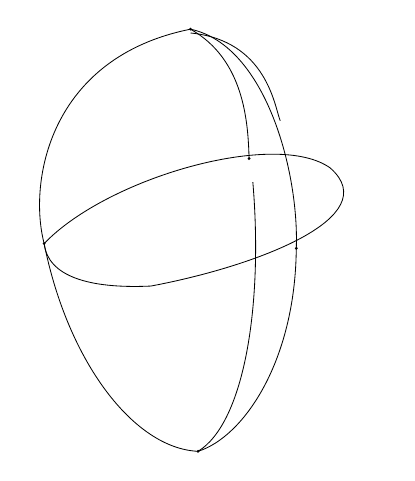
\begin{tikzpicture}[x=.012cm,y=-.012cm,line width=.3pt]
\draw (350,1238) .. controls (200,1268) and (178,1400) .. (195,1465) .. controls (220,1590) and (290,1682) .. (358,1685);
\draw (350,1238) .. controls (430,1255) and (465,1390) .. (462,1470) .. controls (461,1590) and (406,1670) .. (358,1685);
\draw (350,1238) .. controls (407,1270) and (411,1337) .. (412,1375);
\draw (416,1400) .. controls (427,1530) and (407,1655) .. (358,1685);
\draw (350,1242) .. controls (431,1250) and (439,1320) .. (445,1335);
\draw (195,1465) .. controls (262,1395) and (441,1344) .. (498,1385) .. controls (557,1437) and (420,1489) .. (308,1510) .. controls (243,1513) and (199,1500) .. (195,1465);
\foreach \p in {(350,1238),(195,1465),(412,1375),(462,1470),(358,1685)}{\fill \p circle[radius=1.6];}
\end{tikzpicture}}
% lower-left projective-line arrow
\diagram{\begin{tikzcd}[ampersand replacement=\&]\unsure{\mathbb P|P}^{1}_{\overline Q}\&\unsure{\mathbb P|P}^{1}_{\overline Q}\arrow[l,"\varphi"']\end{tikzcd}}
% lower drawing, all labels and repeated pencil arcs retained
\figure{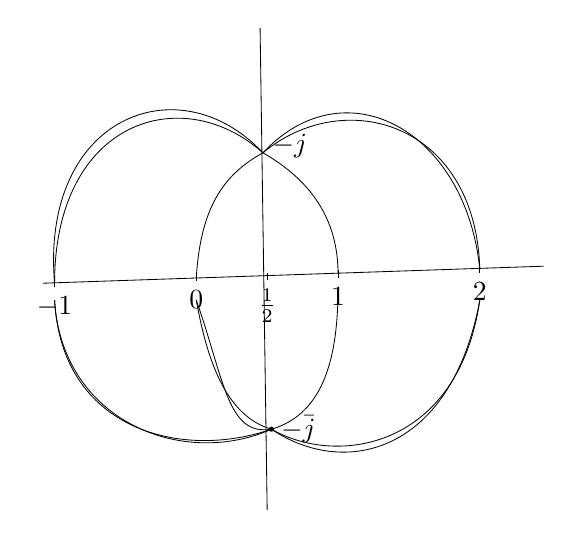
\begin{tikzpicture}[x=1.8cm,y=1.8cm,line width=.3pt]
\draw (-1.08,0)--(2.45,.12);\draw (.5,-1.6)--(.45,1.8);
\draw (-1,0) .. controls (-1,1.15) and (-.1,1.43) .. (.47,.92) .. controls (.89,.68) and (1,.36) .. (1,.065);
\draw (-1,0) .. controls (-1.1,1.18) and (-.12,1.55) .. (.47,.92);
\draw (0,.04) .. controls (.03,.52) and (.18,.76) .. (.47,.92) .. controls (1.05,1.4) and (1.97,1.13) .. (2,.1);
\draw (.47,.92) .. controls (1.05,1.54) and (1.9,1.08) .. (2,.1);
\draw (-1,-.12) .. controls (-.95,-1.04) and (-.1,-1.25) .. (.53,-1.03) .. controls (.91,-.92) and (1,-.5) .. (1,-.03);
\draw (-1,-.12) .. controls (-.95,-.97) and (-.1,-1.31) .. (.53,-1.03);
\draw (0,-.12) .. controls (.08,-.57) and (.22,-.94) .. (.53,-1.03) .. controls (1,-1.3) and (1.85,-1.16) .. (2,-.12);
\draw (0,-.12) .. controls (.2,-.69) and (.22,-1.08) .. (.53,-1.03) .. controls (1.05,-1.38) and (1.8,-1.2) .. (2,-.12);
\foreach \x/\y/\lab in {-1/0/{-1},0/.04/{0},.5/.05/{\frac12},1/.065/{1},2/.1/{2}}{\draw (\x,\y-.025)--(\x,\y+.025);\node[below] at (\x,\y-.025) {$\lab$};}
\fill (.53,-1.03) circle[radius=.018];\node[right] at (.47,.97) {$-j$};\node[right] at (.53,-1.03) {$-\bar j$};
\end{tikzpicture}}
